\iffalse
%-*- program: xelatex -*-        
%-*- program: biber -*-`        
%-*- program: xelatex -*-
\documentclass[12pt]{article}
\usepackage{amsmath,textcomp,amssymb,geometry,graphicx,enumerate,upquote,color}
\usepackage{array}
\usepackage[english]{babel}
\begin{document}

\section{Regime Switching Model}
\fi

Economic time series data tend to behave differently in adjacent time period. For example, asset returns
usually show large volatility during financial crisis. One common approach to model this abrupt change in regime is to use the Hamilton's Markov regime switching model. In our study, we use the following two-regime switching model to fit the returns:

\begin{equation}
y_t - \mu_{s^*_t} = \phi_{s^*_t} (y_{t-1} - \mu_{s^*_{t-1}}) + \epsilon_t
\end{equation}
where the number of autoregressive coefficient is set to 1. $s^*_t$ is a two state Markov chain. $s^*_t = 1$ represent regime 1 and $s^*_t = 2$ represent regime 2. $s^*_t$ depends on the past only through the most recent values:

\begin{equation}
P(s_t = j|s_{t-1}, s_{t-2}, \dots) = P(s_t = j|s_{t-1})  = p_{ij}
\end{equation}

\subsection{Comparison of basic summary of two regimes}

Table \ref{table:autoCoeffRegime} shows the autoregression coefficient $\phi$ of two regimes for various assets. One interesting fact is that asset returns are more likely (6 out of 10 assets) to show positive autocorrelation in low volatility regimes and negative autocorrelation in high volatility regimes.

Table \ref{table:statSumRegime} shows the standard deviation, skewness and kurtosis of various assets in two regimes separately. Note that regime 1 represents high volatility regime while regime 2 represents low volatility regime. In general, it is clear that returns of regime 1 has a larger standard deviation, skewness and kurtosis than that of regime 2. This indicates that the distribution in low volatility regimes are more ``close" to normal distribution. Their mean returns are more close to zero and they have lighter tails than returns of high volatility regime. In contrast, in high volatility regimes, there are more extreme value of returns which means a fatter tail.

\begin{table}[!h]
\caption{$\phi$ of high and low volatility regimes for various assets} 
\centering 
\begin{tabular}{ | c || r  r | } 
 \hline
 & Regime 1  & Regime 2\\
Asset & High volatility  & Low volatility \\
  \hline \hline
AGG  & -0.134 & -0.114 \\ 
HYG & -0.010 &  0.025 \\ 
TIP &  0.039  & -0.026 \\ 
BCOM & -0.046 &  0.050 \\ 
MXEA & 0.095 & 0.109 \\ 
MXEF & 0.221 & 0.254 \\ 
RAY& -0.039  &  0.052 \\ 
RMZ & -0.244 &  0.007 \\ 
SPX & -0.018 &  0.113 \\ 
USGG10YR & -0.031 & 0.082 \\ 
 \hline
\end{tabular}
\label{table:autoCoeffRegime}
\end{table}

\begin{table}[!h]
\caption{Summary statistics of two regimes for various assets} 
\centering 
\begin{tabular}{ | c || rr | rr | rr | } 
 \hline
& \multicolumn{2}{c|}{Volatility} & \multicolumn{2}{c|}{Skewness} & \multicolumn{2}{c|}{Kurtosis} \\
Asset & Regime 1 & Regime 2 & Regime 1 & Regime 2 & Regime 1 & Regime 2 \\
  \hline \hline
AGG & 0.141 & 0.036 & -1.59 &  0.01 & 17.15 &  0.60\\ 
HYG & 0.265 & 0.055 &  0.60 &  0.00 &  8.76 &  0.83\\ 
TIP & 0.113 & 0.049 &  0.18 & -0.06 &  2.50 &  0.16\\ 
BCOM & 0.205 & 0.096 & -0.25 & -0.04 &  1.92 &  0.28\\ 
MXEA & 0.253 & 0.101 & -0.14 & -0.02 &  4.26 &  0.25\\ 
MXEF & 0.303 & 0.119 & -0.08 & -0.06 &  2.39 &  0.38\\ 
RAY & 0.307 & 0.114 & -0.39 & -0.06 &  6.43 &  0.55\\ 
RMZ & 0.661 & 0.159 &  0.29 & -0.15 &  2.92 &  0.79\\ 
SPX & 0.260 & 0.099 & -0.43 & -0.02 &  9.11 &  0.56\\ 
USGG10YR & 0.314 & 0.098 &  0.09 & -0.05 &  2.67 &  1.17 \\
 \hline
\end{tabular}
\label{table:statSumRegime}
\end{table}

\subsection{Detailed analysis (Take RMZ as an example)}

\subsubsection{Summary}

In Figure \ref{fig: RMZregime}, we use RMZ as an example of our volatility regime analysis. The upper panel show the daily returns and their corresponding regimes. The shadowed area represents the regime with high volatility and the white area low volatility. The X axis shows the indices of business days from 06/30/2005 to 12/31/2015. The lower panel shows the smoothed probability of Markov switching model corresponds with the high volatility regime. This model is consistent with the actual financial event in that the high volatility regime covered mainly from mid-2007 to 2010, which is roughly the period of 2008-09 financial crisis.

Table \ref{table:statSumRegimeRMZ} shows the descriptive summary and risk diagnostics for RMZ of each regime. As we might expect, regime with high volatility also shows high risks in that they have larger ES and VaR values. Moreover, model of regime 1 only explains 26.3\% of the observations, which means abrupt deviation is minority in total observations. By looking at assets with longer period, we find a similar proportion of high volatility regimes (SPX: 23.7\%, RAY: 20.6\%).

%\begin{figure}[h]
%\caption{Regime plot of SPX returns and its smoothed probabilities} 
%\centering 
%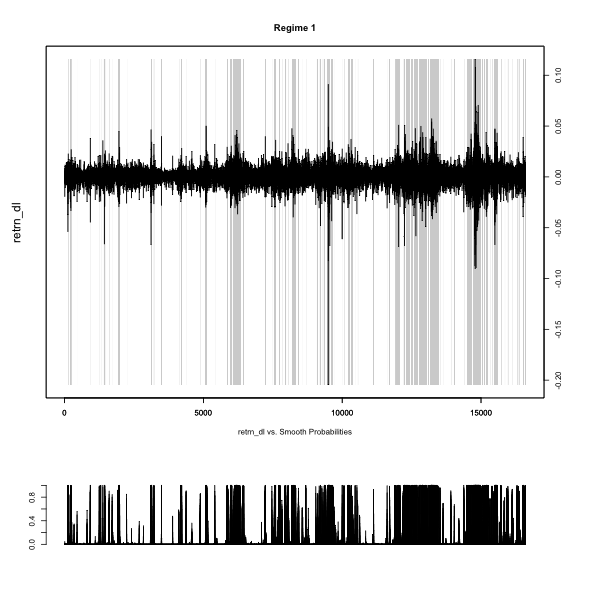
\includegraphics[width=1\textwidth]{../results/regime/SPX}
%\label{fig: returnsDist}
%\end{figure}

\begin{figure}[h]
\caption{Regime plot of RMZ returns and its smoothed probabilities} 
\centering 
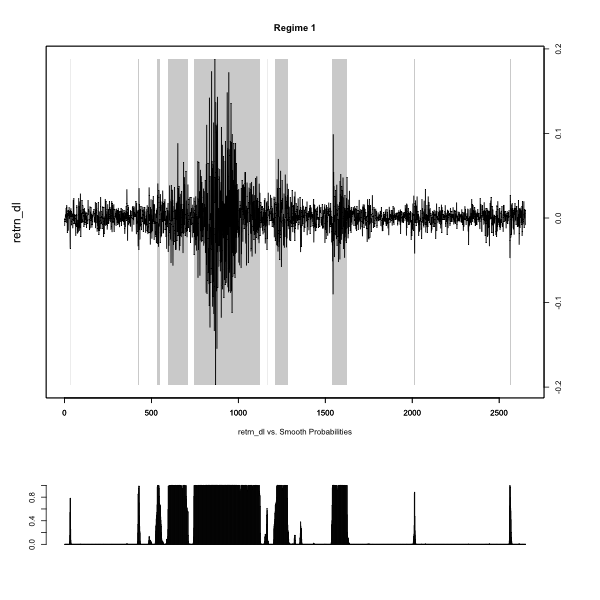
\includegraphics[width=1\textwidth]{../results/regime/RMZ}
\label{fig: RMZregime}
\end{figure}

\begin{table}[h]
\caption{Descriptive summary and risk diagnostics for RMZ of each regime} 
\centering 
\begin{tabular}{| r | r | r |} 
 \hline
& Regime 1 & Regime 2 \\
& High volatility & Low volatility \\
 \hline 
Mean & -0.046\% & 0.067\% \\
Number of trading days & 699 & 1954\\ 
Percentage of observations & 26.3\% & 73.7\% \\ 
Maximum daily return &18.8\% & 3.6\% \\
Minimum daily return & -19.7\% & -4.0\% \\
Longest continuous days & 381 & 546\\ \hline
VaR (empirical, p = 0.95) & 6.8\% & 1.6\% \\
ES (empirical, p = 0.95) & 9.3\% & 2.2\% \\
 \hline
\end{tabular}
\label{table:statSumRegimeRMZ}
\end{table}

\subsubsection{Risk diagnostics}

In order to make a consistent comparison of risk diagnostics between two regimes, we ignore some short discontinuity and pick two longest single occurring episode for each regime. Both episode contain 530 trading days. The episode of regime 1 range from 10/30/2007 to 12/07/2009, and the episode of regime 2 range from 06/20/2013 to 07/29/2015.

As shown in Table \ref{table:ridkDiagsRegimeRMZ}, The episode of regime 1 have significantly larger VaR, ES and CED value, which indicate a larger risk. This is consistent with the fact that returns of regime 1 have larger volatility. Figure \ref{fig: RMZregime_mdd} shows the maximum drawdown distribution of now-month rolling window. It is clear from the figure that regime 1 with higher volatility has larger maximum drawdown values than regime 2. We further look at the summary statistics of the two regimes and compare them with the overall drawdown distribution in Table \ref{table:SummatyMDDRegimeRMZ}. After dividing them into two regimes, both knewness and kurtosis declined. The regime with high volatility has larger mean, standard deviation, skewness and kurtosis. For the case of RMZ, The regime with high risk also have a higher serial correlation for order one and order two. 

\begin{table}[h]
\caption{Risk diagnostics for RMZ of two equal-length episode of each regime} 
\centering 
\begin{tabular}{| r | r | r |} 
 \hline
& Regime 1 & Regime 2 \\
& High volatility & Low volatility \\
 \hline 
VaR (empirical, p = 0.95) & 7.4\% & 1.5\% \\
ES (empirical, p = 0.95) & 9.9\% & 2.1\% \\
CED (one-month, p = 0.9) & 38.4\% & 8.4\% \\
Serial correlation (order = 1) & -0.257 & -0.026 \\
Serial correlation (order = 2) & -0.023 & 0.008 \\
 \hline
\end{tabular}
\label{table:ridkDiagsRegimeRMZ}
\end{table}

\begin{table}[h]
\caption{Summary statistics of maximum drawdown distribution} 
\centering 
\begin{tabular}{| r | r | r | r |} 
 \hline
& Regime 1 & Regime 2 & \\
& High volatility & Low volatility & Overall \\
 \hline 
Mean & 0.14 & 0.04 & 0.07\\
Medium  & 0.11 & 0.03 & 0.049 \\
Max  & 0.47 & 0.13 & 0.47\\
Standard diviation & 0.10 & 0.02 & 0.07\\
Sknewness & 1.60 & 1.06 & 2.86\\
Kurtosis  & 1.87 & 1.12 & 10.9\\
 \hline
\end{tabular}
\label{table:SummatyMDDRegimeRMZ}
\end{table}


\begin{figure}[h]
\caption{Maximum drawdown density of two regimes} 
\centering 
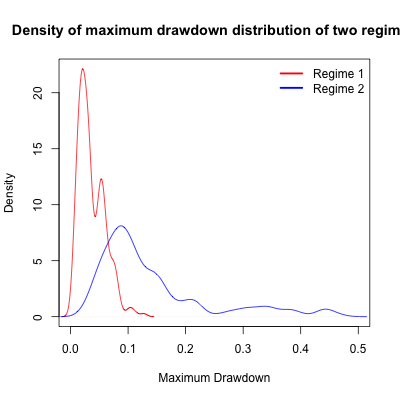
\includegraphics[width=0.7\textwidth]{../results/regime/RMZ_mon1_mdd}
\label{fig: RMZregime_mdd}
\end{figure}

\subsubsection{Rolling risk diagnostics}

For the two regimes in the above section, we calculated the VaR, ES, VaR and maximum drawdown based on one-month rolling window. Based on the rolling risk diagnotics, we are able to calculate and compare the corelation between different risk diagnotics and their difference under high and low volatility regimes. As shown in Table \ref{table:corr_risk_serial_regime}, in high volatility regimes, the correlation between isk diagnostics and serial correlation is higher than in low volatility regimes.

\begin{table}[!h]
\caption{correlation between risk diagnostics and serial correlation of two equal-length episode of each regime} 
\centering 
\begin{tabular}{| r | r | r |} 
 \hline
& Regime 1 & Regime 2 \\
& High volatility & Low volatility \\
 \hline 
corr(VaR, $\rho(1)$)  & -0.29 & 0.08 \\
corr(ES, $\rho(1)$)   & -0.30 & 0.07 \\
corr(volatility, $\rho(1)$)  & -0.33 & 8.4 \\
corr(maximum drawdown, $\rho(1)$)  & -0.24 & 0.07 \\
 \hline
\end{tabular}
\label{table:corr_risk_serial_regime}
\end{table}

\iffalse
\end{document}
\fi